\documentclass[11pt]{article}
\usepackage[margin=0.7in]{geometry}
\usepackage{booktabs,amsmath,amssymb,graphicx,subcaption}
\newcommand{\sym}[1]{\ifmmode^{#1}\else\(^{#1}\)\fi}
\setlength{\parindent}{0pt}
\begin{document}
\begin{center}\large\textbf{Risk-preference similarity: group CCEI and CEIV}\end{center}
\begin{center}\small
\begin{tabular}{lccc}\toprule
& Full sample & Similar risk preferences & Different risk preferences\\
& & Below wave median & Above wave median\\
\midrule
\multicolumn{4}{l}{\textit{Group CCEI -- OLS}}\\
$\text{CCEI}_{\text{max},gt}$&    0.131        &    0.056        &    0.200        \\
                &  (0.095)        &  (0.130)        &  (0.122)        \\
$\text{CCEI}_{\text{min},gt}$&    0.235\sym{**}&    0.252\sym{**}&    0.221\sym{**}\\
                &  (0.045)        &  (0.061)        &  (0.059)        \\
\midrule
N               &     1304        &      652        &      652        \\
R-squared       &    0.197        &    0.238        &    0.254        \\
\midrule
\multicolumn{4}{l}{\textit{Group CEIV -- OLS}}\\
$\text{CCEI}_{\text{max},gt}$&    0.176\sym{+} &    0.064        &    0.296\sym{*} \\
                &  (0.094)        &  (0.099)        &  (0.136)        \\
$\text{CCEI}_{\text{min},gt}$&    0.086\sym{*} &    0.064\sym{+} &    0.074        \\
                &  (0.035)        &  (0.037)        &  (0.051)        \\
\midrule
N               &     1304        &      652        &      652        \\
R-squared       &    0.115        &    0.179        &    0.191        \\

Class fixed effects & $\checkmark$ & $\checkmark$ & $\checkmark$\\
Student and friendship controls & $\checkmark$ & $\checkmark$ & $\checkmark$\\
Corner/midpoint share controls & $\checkmark$ & $\checkmark$ & $\checkmark$\\
\bottomrule
\end{tabular}\end{center}
\small
\textit{Notes:} Reproduces Table 5 column (3) for group CCEI and CEIV, separately
by similarity of the members' individually revealed risk preferences.
The gap is $|RA_i-RA_j|$, where $RA_m$ is the member's mean share of the allocation
to the more expensive security over her 18 individual choices in that wave.
The median is computed across 652 pairs separately within each wave:
0.109252 at baseline and 0.145095 at endline. There are no missing gaps or median ties. Each subgroup contains 326
pair-waves per wave, totaling 652; pairs can switch subgroups across waves.
All models include both individual CCEIs, class fixed effects, and the original
student, friendship, and corner/midpoint-share controls. Risk-aversion controls
are excluded, matching column (3). Standard errors are clustered by 64 classes
and reported in parentheses. +, *, and ** indicate $p<0.10$, $p<0.05$, and $p<0.01$.

\medskip
\textbf{Tests of subgroup coefficient differences}\par
\begin{center}
\begin{tabular}{llrr}\toprule
Outcome & Individual CCEI & Above minus below & $p$-value\\\midrule
CCEI & $\text{CCEI}_{\text{max}}$ & 0.144 & 0.436\\
CCEI & $\text{CCEI}_{\text{min}}$ & -0.031 & 0.727\\
CEIV & $\text{CCEI}_{\text{max}}$ & 0.232 & 0.179\\
CEIV & $\text{CCEI}_{\text{min}}$ & 0.010 & 0.880\\
\bottomrule\end{tabular}\end{center}
\textit{Notes:} Class-clustered Wald tests from a pooled OLS regression that fully
interacts subgroup membership with all regressors and class fixed effects.
These tests account for dependence across the two subgroups within a class.
Differences in significance across separate models alone do not establish
significant heterogeneity. The risk-preference split is descriptive and uses
the same individual choices used to measure individual CCEI.
\clearpage
\begin{center}\large\textbf{Figure 6: group CCEI and CEIV}\par
\normalsize Similar risk preferences: below the wave median\end{center}
\begin{figure}[ht]\centering
\begin{subfigure}[b]{0.485\textwidth}\centering
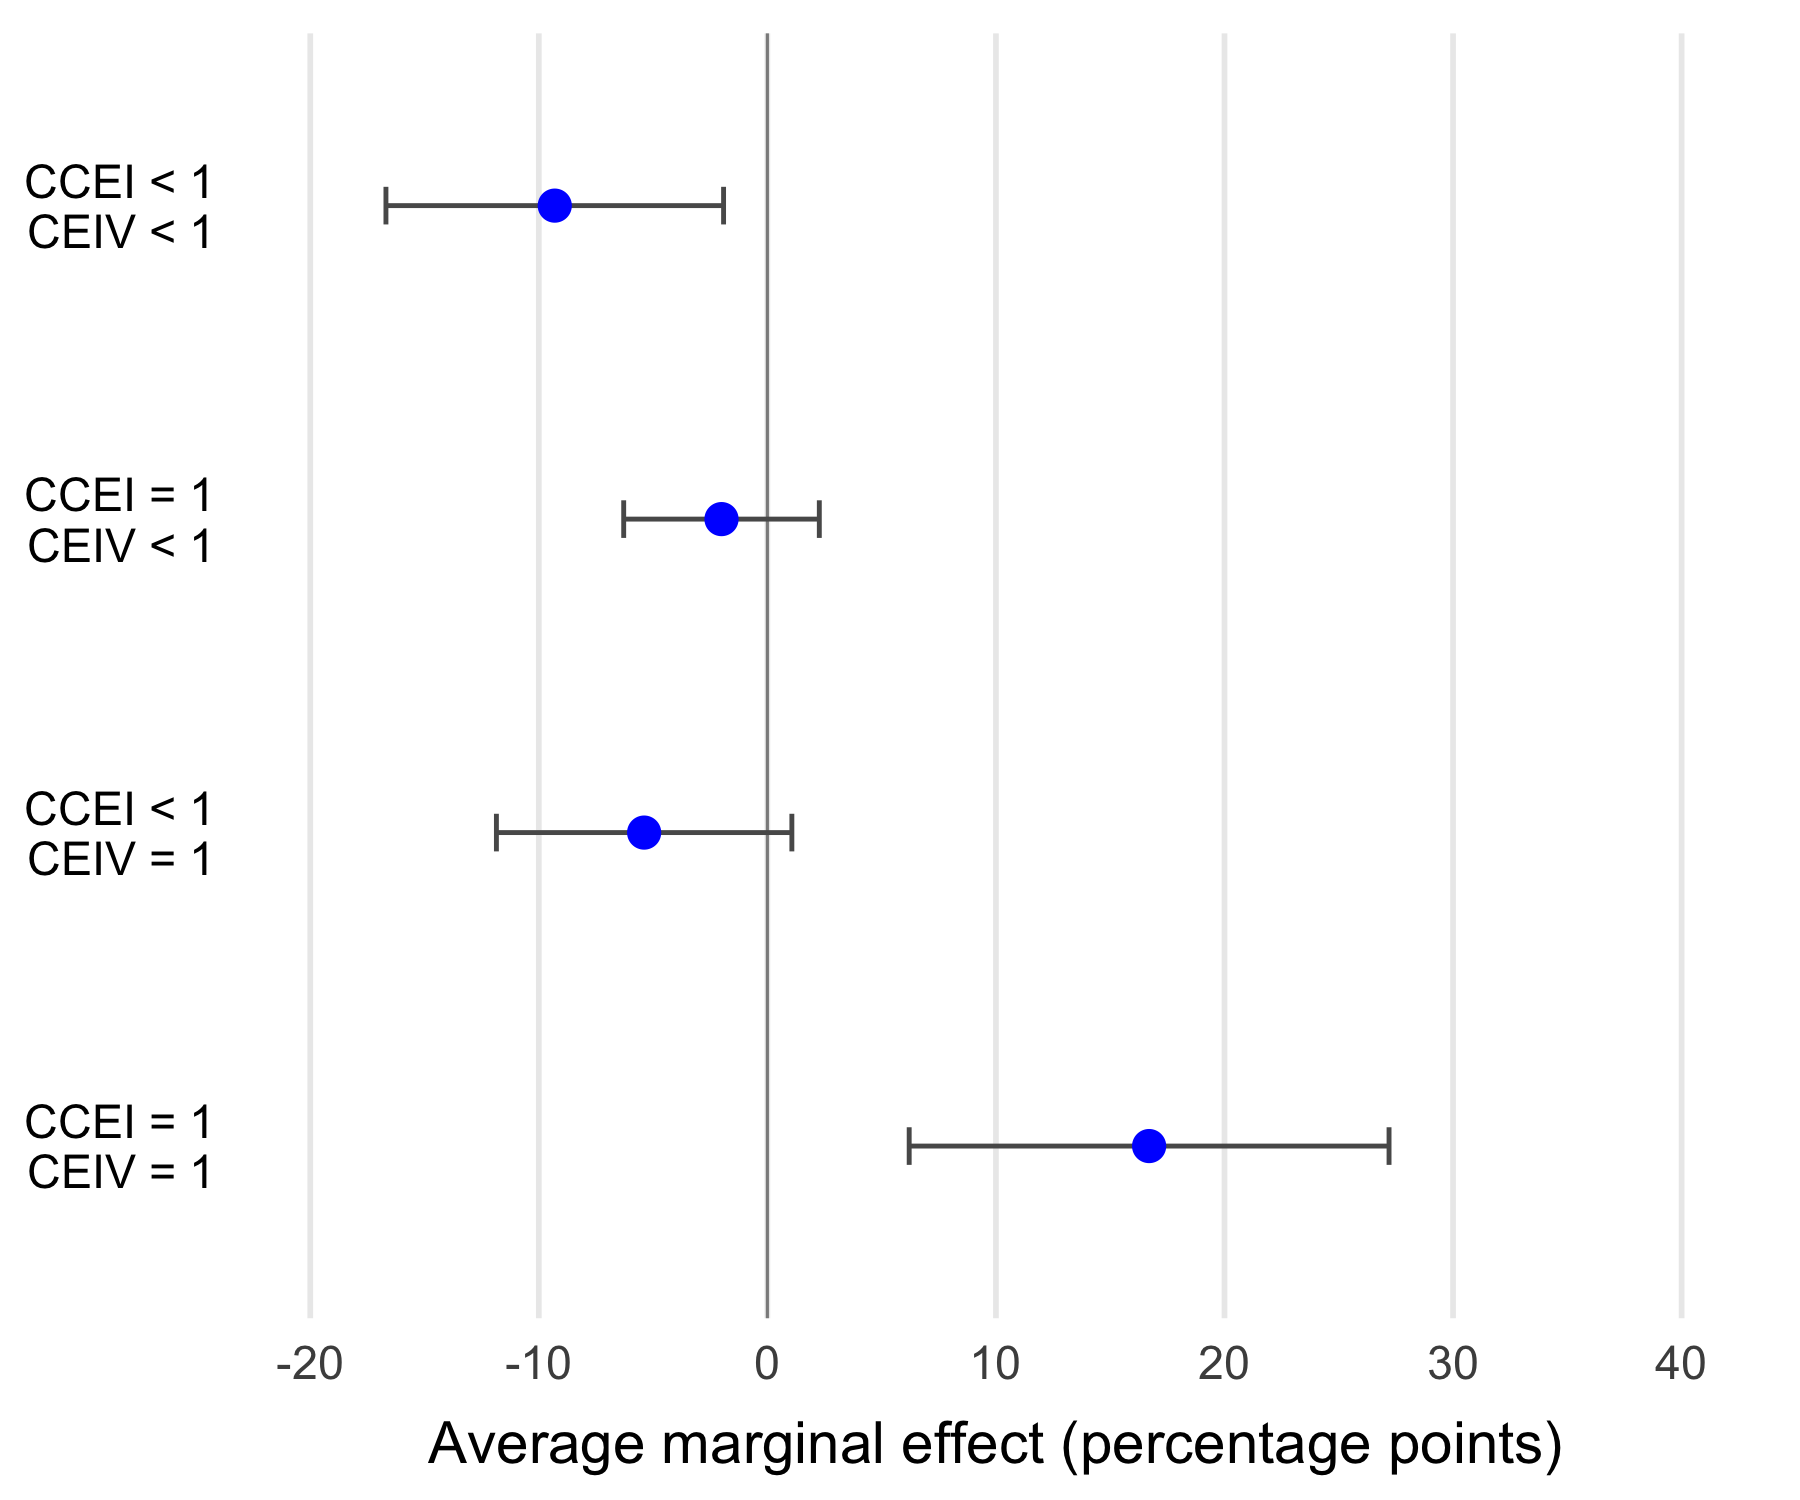
\includegraphics[width=\textwidth]{figure6_a_similar_ame_maximum.png}
\caption{$\text{CCEI}_{\text{max},gt}$}\end{subfigure}\hfill
\begin{subfigure}[b]{0.485\textwidth}\centering
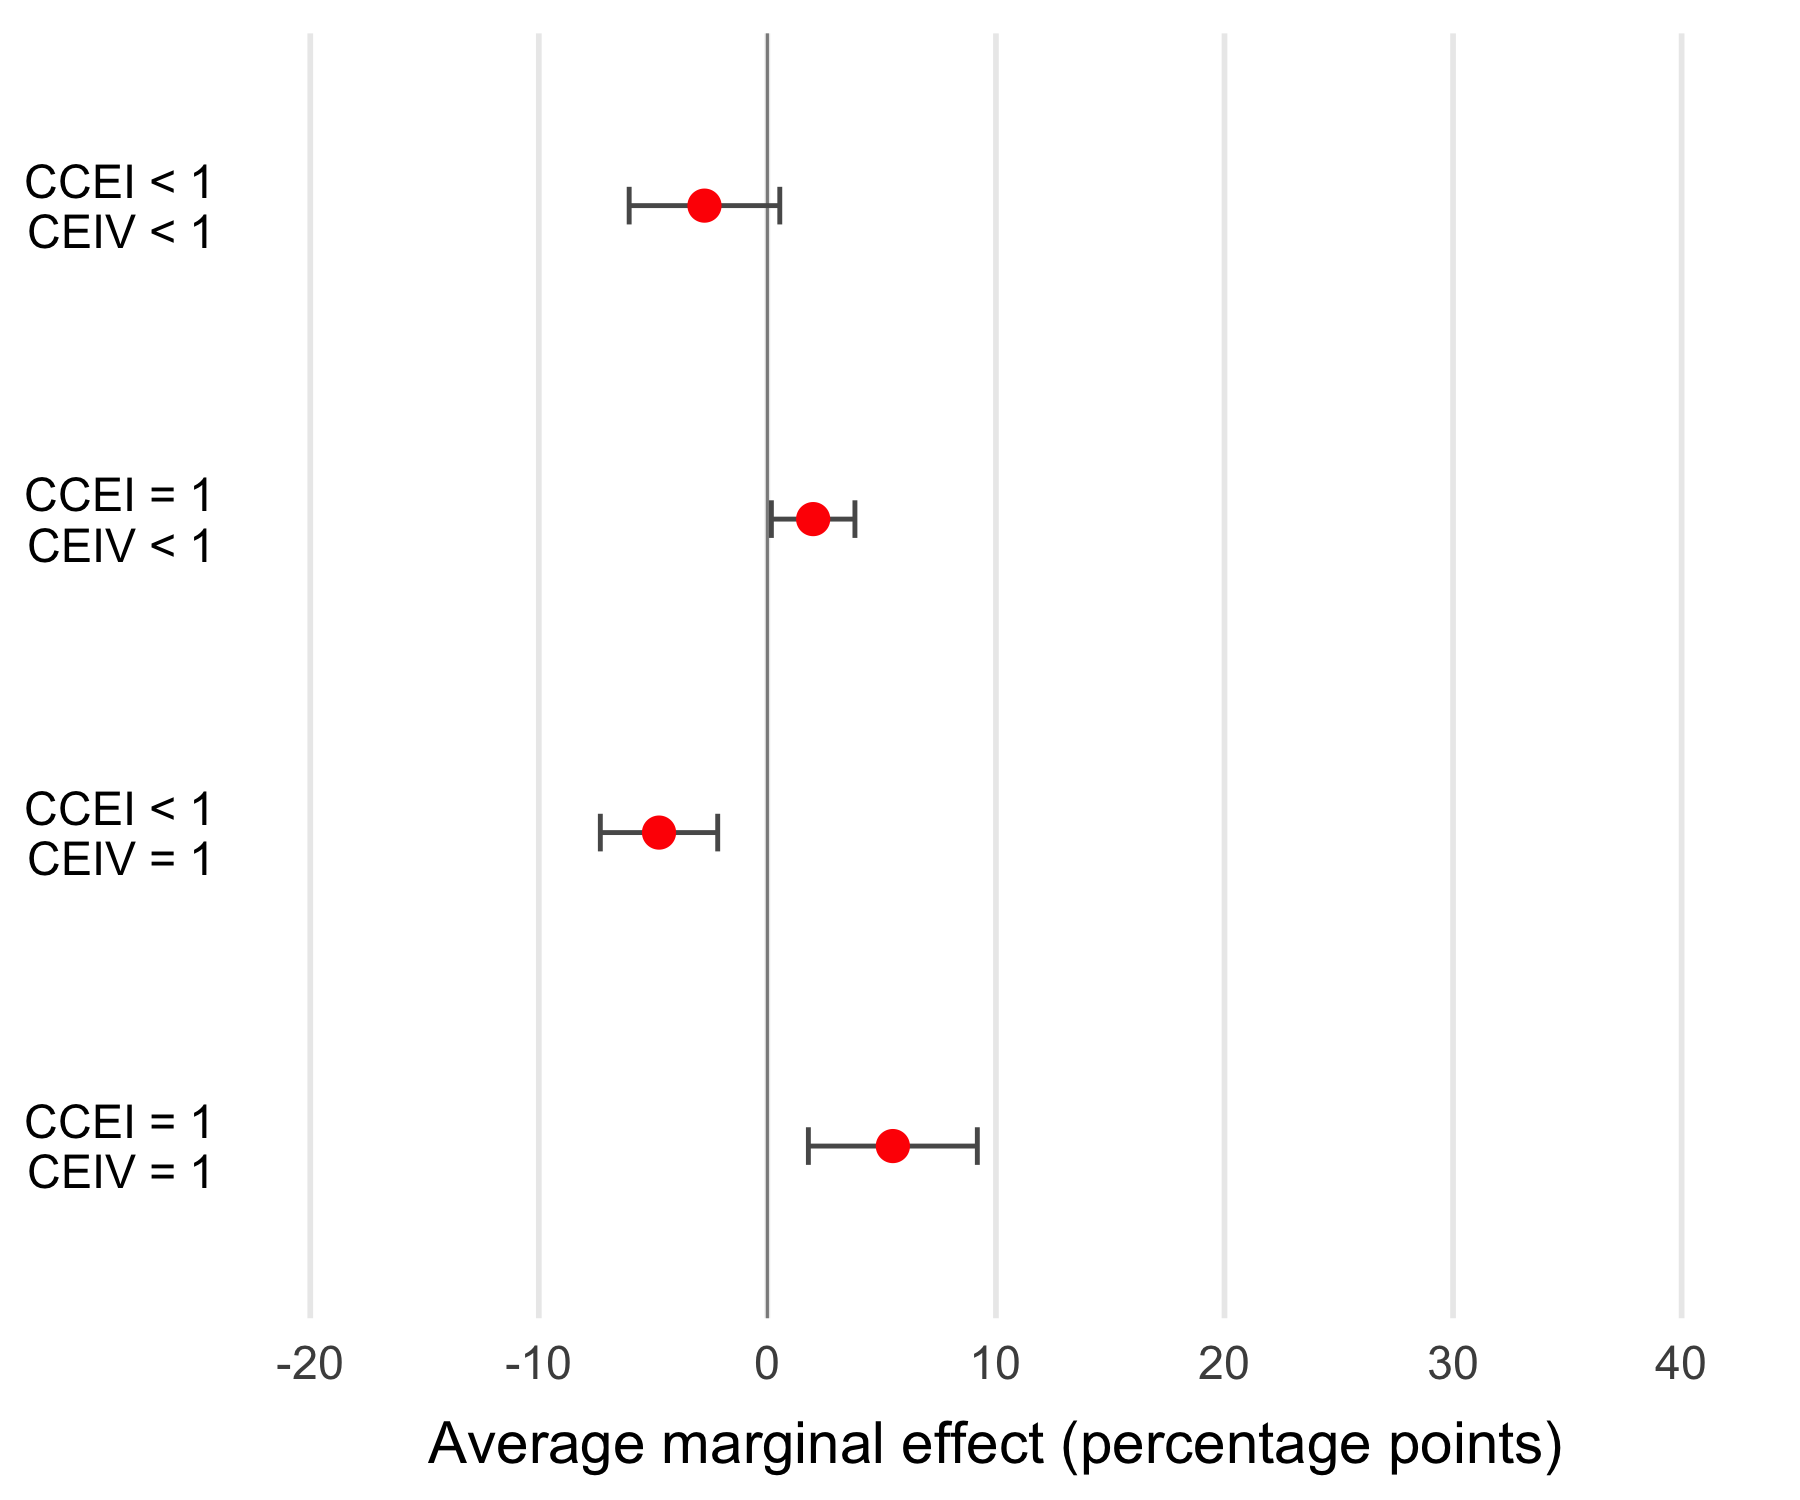
\includegraphics[width=\textwidth]{figure6_a_similar_ame_minimum.png}
\caption{$\text{CCEI}_{\text{min},gt}$}\end{subfigure}
\end{figure}
\small
\textit{Notes:} Separate four-category multinomial-logit model in the indicated
risk-preference-gap subgroup, using Table 5 column (3)'s controls and class fixed
effects. Both maximum and minimum individual CCEI enter jointly. Risk-aversion
controls are excluded. Plotted average marginal effects are in percentage points
for a 0.1 increase in individual CCEI; they are scaled average derivatives,
not exact finite probability changes. Error bars are 95\% confidence intervals
using class-clustered standard errors.

\medskip
Sample: 652 pair-waves from 462 distinct pairs in 64 classes.
The gap $|RA_i-RA_j|$ is classified within each wave using medians 0.109252 and 0.145095;
there are 326 observations per wave in this subgroup.
Category shares, from top to bottom: 34.51\%, 8.59\%, 23.16\%, 33.74\%.
Classification uses the supplied indices and the original $10^{-9}$ tolerance;
CEIV classifications are unchanged across their supplied numerical bounds.
Both subgroup figures use a common horizontal scale covering all confidence
intervals. The blue/red member colors and panel styling follow Figure 6.
\clearpage
\begin{center}\large\textbf{Figure 6: group CCEI and CEIV}\par
\normalsize Different risk preferences: above the wave median\end{center}
\begin{figure}[ht]\centering
\begin{subfigure}[b]{0.485\textwidth}\centering
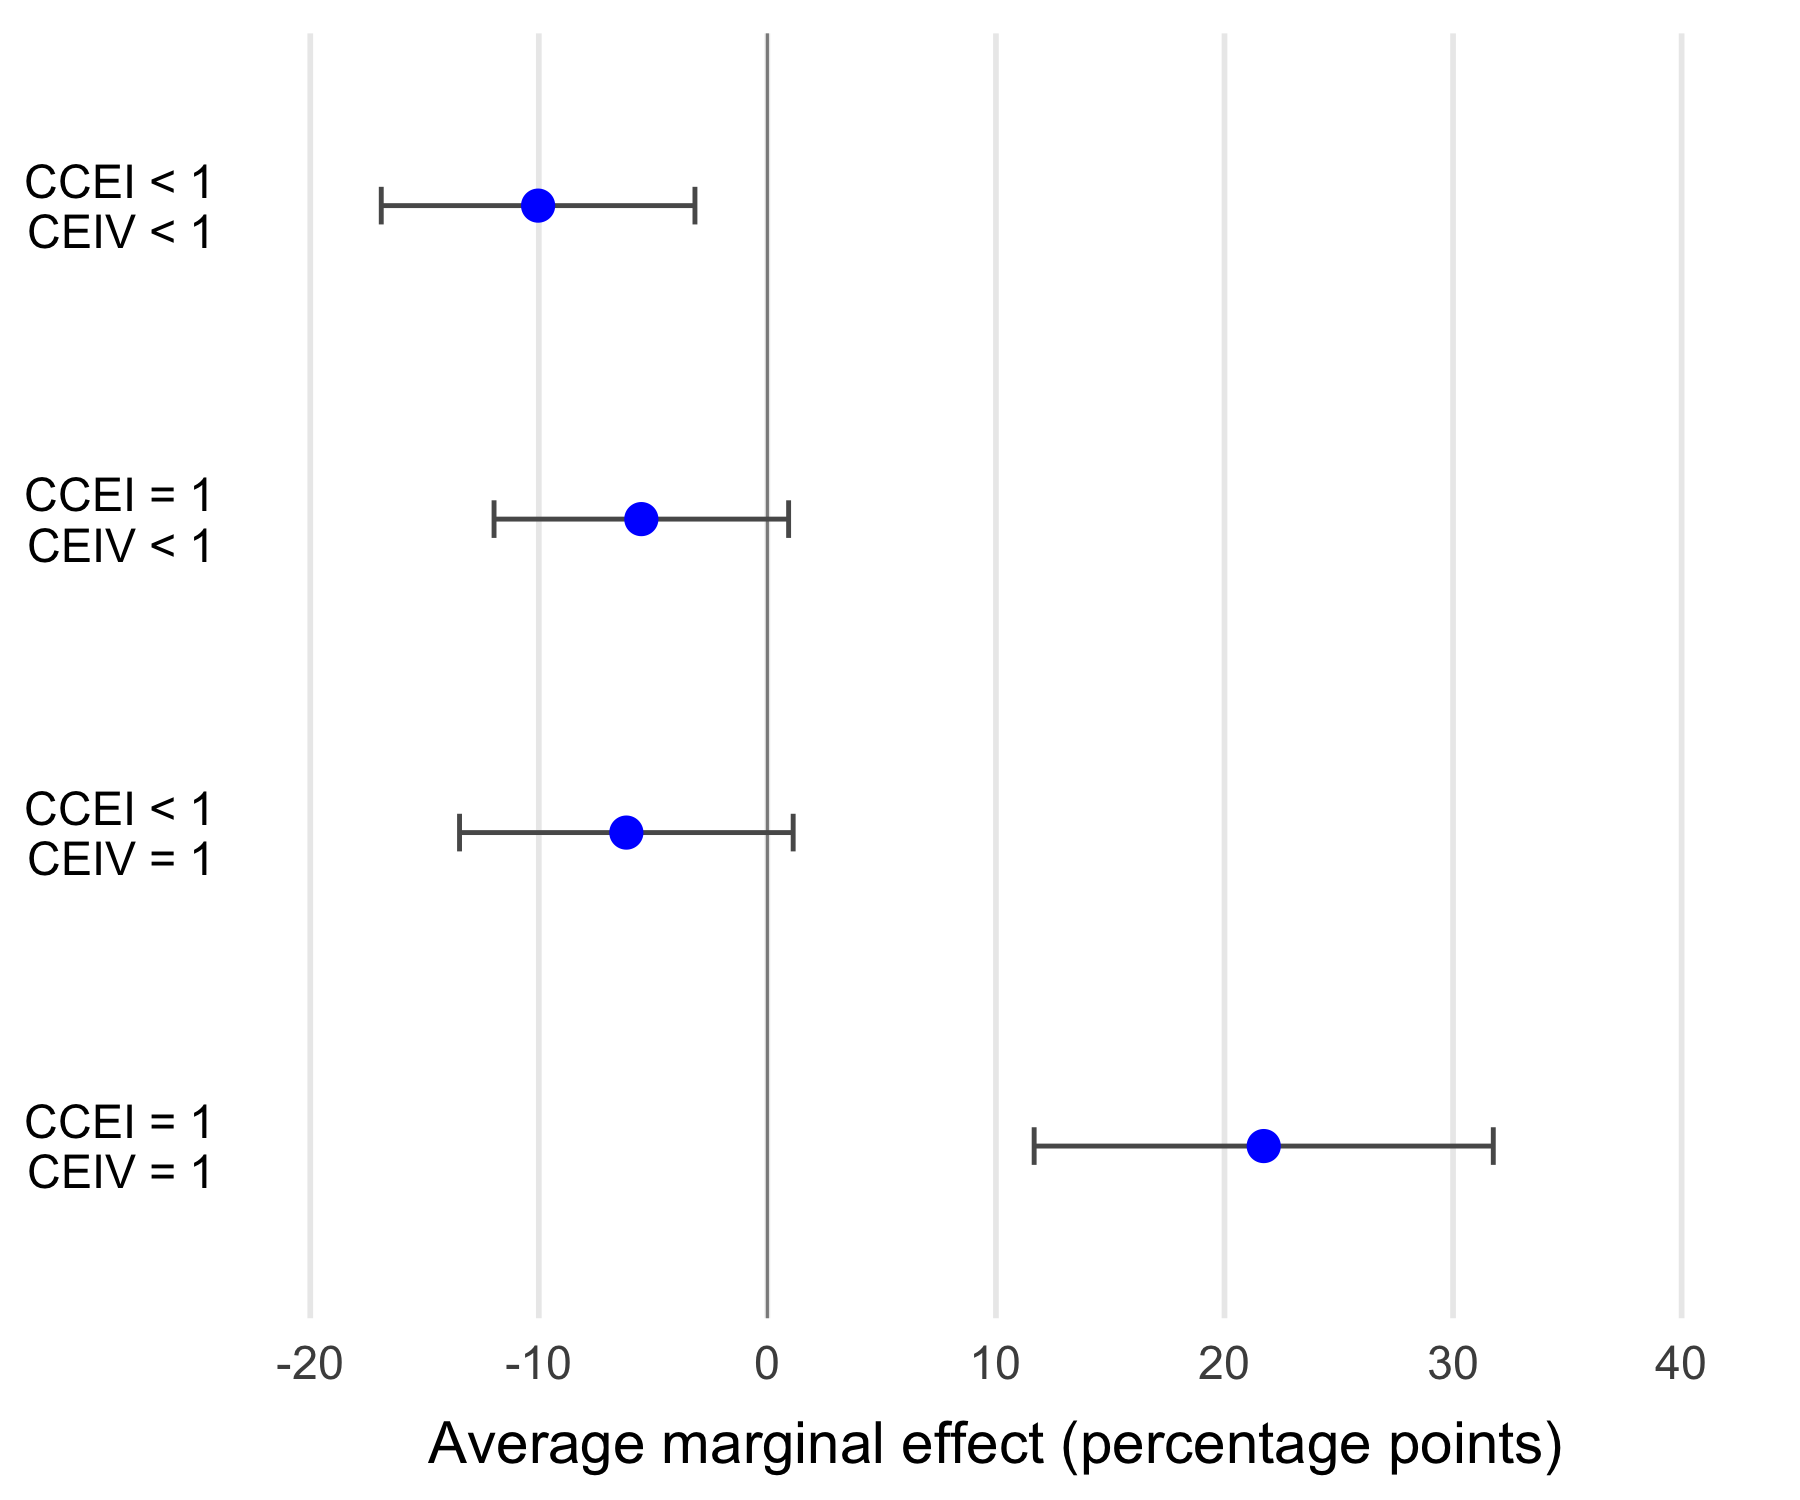
\includegraphics[width=\textwidth]{figure6_a_different_ame_maximum.png}
\caption{$\text{CCEI}_{\text{max},gt}$}\end{subfigure}\hfill
\begin{subfigure}[b]{0.485\textwidth}\centering
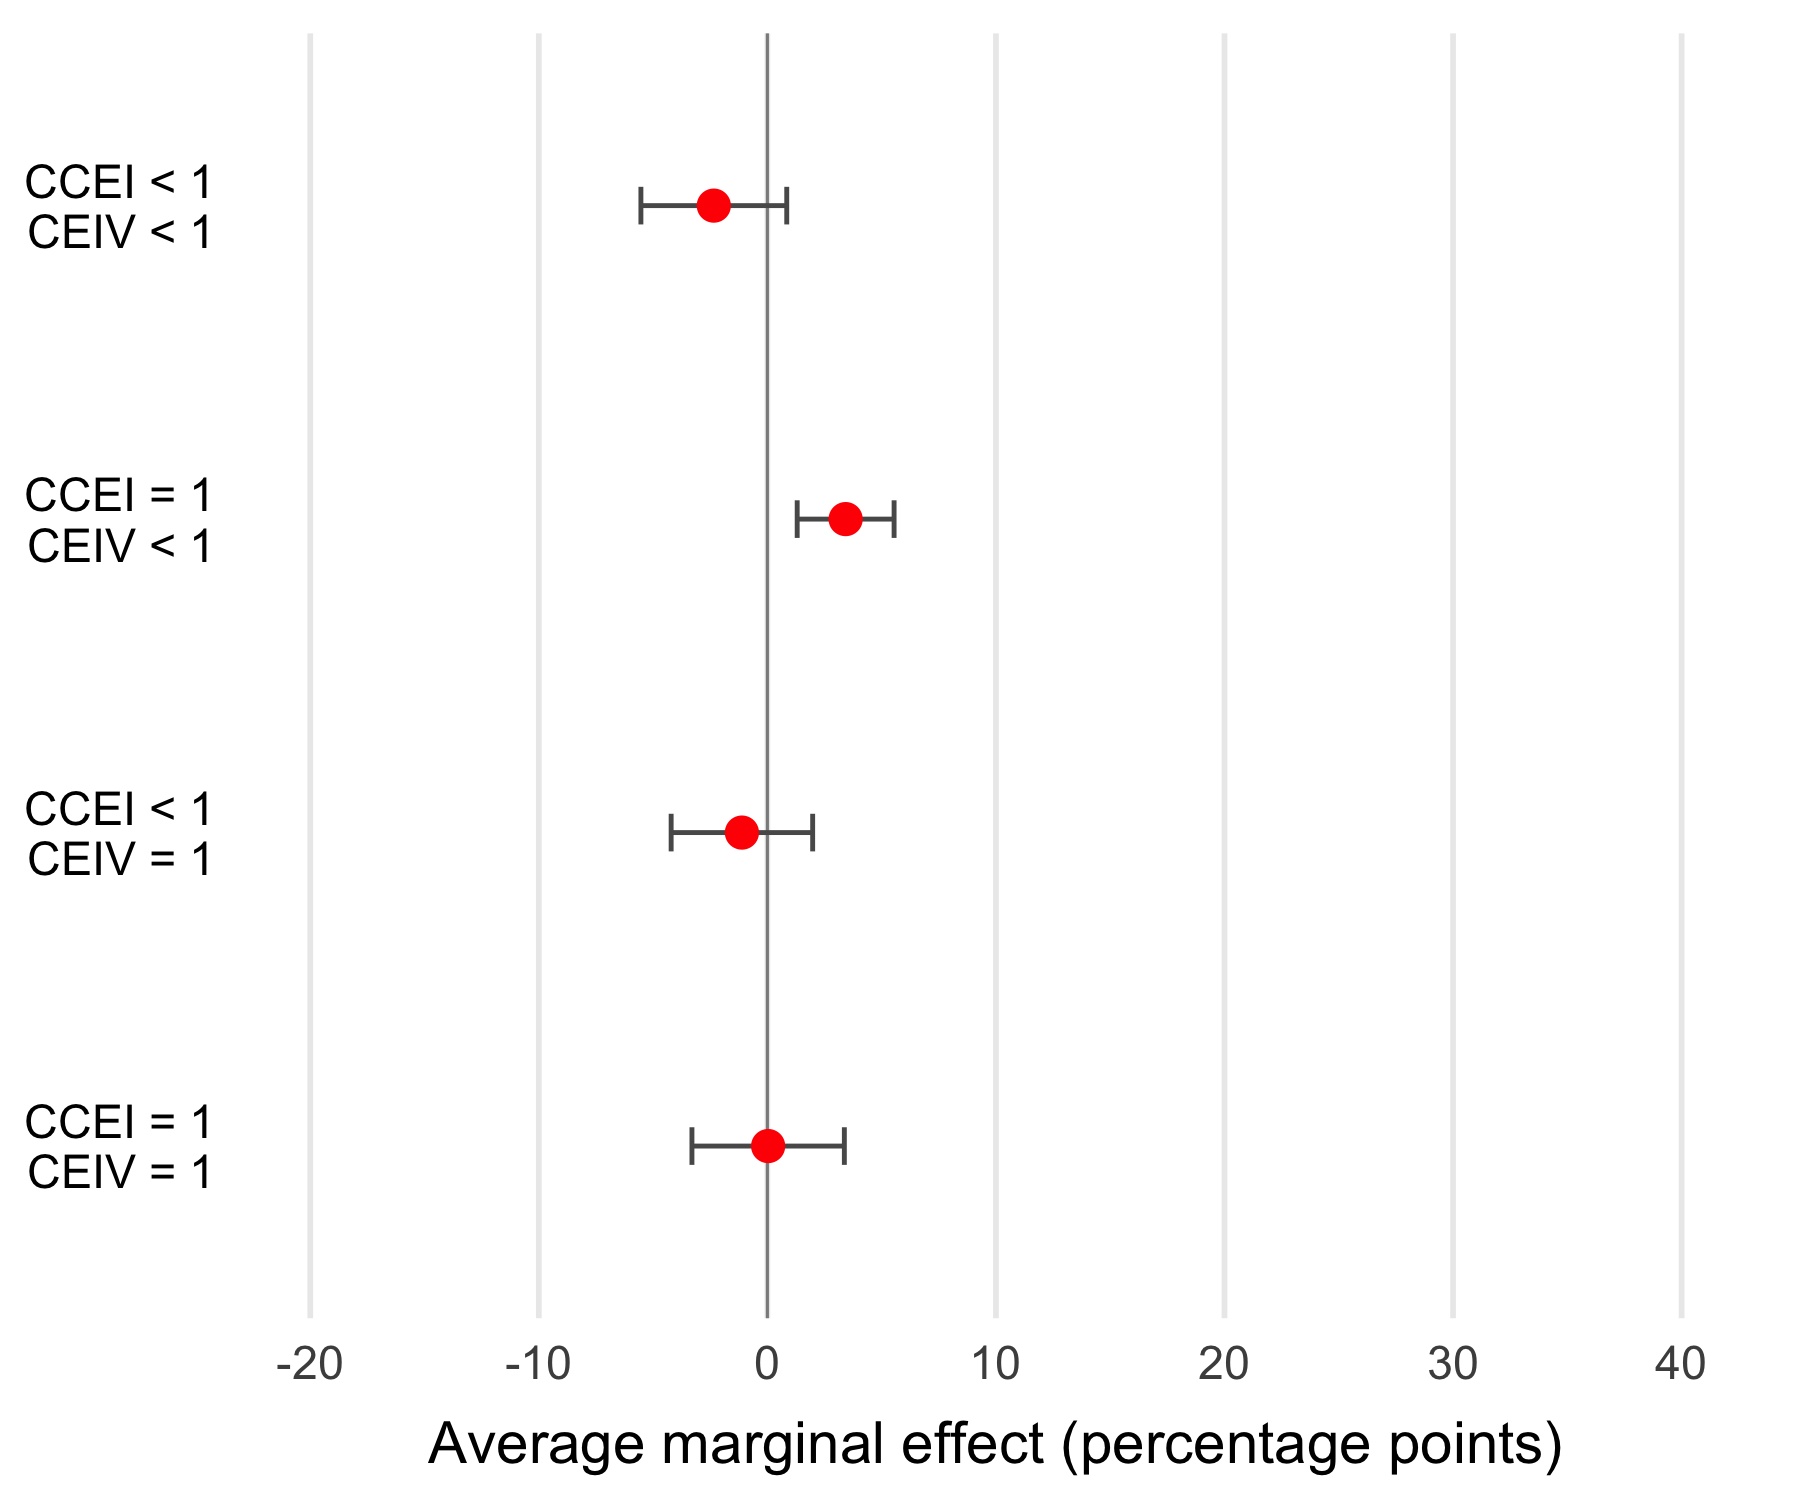
\includegraphics[width=\textwidth]{figure6_a_different_ame_minimum.png}
\caption{$\text{CCEI}_{\text{min},gt}$}\end{subfigure}
\end{figure}
\small
\textit{Notes:} Separate four-category multinomial-logit model in the indicated
risk-preference-gap subgroup, using Table 5 column (3)'s controls and class fixed
effects. Both maximum and minimum individual CCEI enter jointly. Risk-aversion
controls are excluded. Plotted average marginal effects are in percentage points
for a 0.1 increase in individual CCEI; they are scaled average derivatives,
not exact finite probability changes. Error bars are 95\% confidence intervals
using class-clustered standard errors.

\medskip
Sample: 652 pair-waves from 462 distinct pairs in 64 classes.
The gap $|RA_i-RA_j|$ is classified within each wave using medians 0.109252 and 0.145095;
there are 326 observations per wave in this subgroup.
Category shares, from top to bottom: 29.14\%, 9.36\%, 22.85\%, 38.65\%.
Classification uses the supplied indices and the original $10^{-9}$ tolerance;
CEIV classifications are unchanged across their supplied numerical bounds.
Both subgroup figures use a common horizontal scale covering all confidence
intervals. The blue/red member colors and panel styling follow Figure 6.
\end{document}
